\documentclass[12pt, a4paper]{report}

% ─── Packages ───────────────────────────────────────────────────────────────
\usepackage[a4paper, margin=1in]{geometry}
\usepackage{graphicx}
\usepackage{booktabs}
\usepackage{array}
\usepackage{longtable}
\usepackage{float}
\usepackage{amsmath}
\usepackage{hyperref}
\usepackage{caption}
\usepackage{subcaption}
\usepackage{setspace}
\usepackage{fancyhdr}
\usepackage{titlesec}
\usepackage{xcolor}
\usepackage{listings}
\usepackage{enumitem}
\usepackage{parskip}
\usepackage{tocloft}
\usepackage{indentfirst}

% ─── Hyperlink setup ────────────────────────────────────────────────────────
\hypersetup{
    colorlinks=true,
    linkcolor=black,
    urlcolor=blue,
    citecolor=black
}

% ─── Header / Footer ────────────────────────────────────────────────────────
\pagestyle{fancy}
\fancyhf{}
\rhead{Material Informatics for Graphene Research Using NLP}
\lhead{}
\cfoot{\thepage}
\renewcommand{\headrulewidth}{0.4pt}

% ─── Code listing style ─────────────────────────────────────────────────────
\lstset{
    basicstyle=\ttfamily\small,
    backgroundcolor=\color{gray!10},
    frame=single,
    breaklines=true,
    keywordstyle=\color{blue},
    commentstyle=\color{gray},
    stringstyle=\color{orange!80!black},
    showstringspaces=false,
    language=Python
}

% ─── Line spacing ───────────────────────────────────────────────────────────
\onehalfspacing

% ════════════════════════════════════════════════════════════════════════════
\begin{document}

% ─── Title Page ─────────────────────────────────────────────────────────────
\begin{titlepage}
    \centering
    \vspace*{1cm}

    {\Large \textbf{Amrita Vishwa Vidyapeetham}}\\[0.3cm]
    {\large Amrita School of Engineering, Coimbatore}\\[0.2cm]
    {\large Department of Artificial Intelligence and Data Science}\\[2cm]

    \rule{\textwidth}{1.5pt}\\[0.4cm]
    {\LARGE \textbf{Material Informatics for Graphene Research\\[0.3cm] Using Natural Language Processing}}\\[0.3cm]
    {\large \textit{A Case Study on Fine-Tuning Transformer-Based LLMs}}\\[0.2cm]
    \rule{\textwidth}{1.5pt}\\[2cm]

    {\large \textbf{Project Report}}\\[0.3cm]
    {\normalsize Submitted in partial fulfilment of the requirements for}\\[0.1cm]
    {\normalsize the 2nd Semester Project}\\[2cm]

    \begin{tabular}{ll}
        \textbf{Author:}     & T. Muthu Raam \\[0.3cm]
        \textbf{Programme:}  & B.Tech -- Artificial Intelligence and Data Science \\[0.3cm]
        \textbf{Batch:}      & 2024--2028 \\[0.3cm]
        \textbf{Supervised by:} & Dr. Kritesh K. Gupta \\
                             & Assistant Professor, School of AI \\
                             & Center for Computational Engineering and Networking (CEN) \\
    \end{tabular}

    \vfill
    {\large April 2025}
\end{titlepage}

% ─── Abstract ───────────────────────────────────────────────────────────────
\chapter*{Abstract}
\addcontentsline{toc}{chapter}{Abstract}

This project investigates the acceleration of material science discoveries through Natural Language Processing (NLP), with a specific focus on graphene --- a two-dimensional (2D) material renowned for its extraordinary strength, high electrical conductivity, and wide-ranging applications in electronics, energy storage, and biomedicine.

Four transformer-based language models --- BART-Base, DistilBART-CNN, Pegasus-XSUM, and T5-Small --- were fine-tuned on a custom-built dataset comprising graphene-related scientific abstracts and corresponding question-answer (Q\&A) pairs sourced from the Scopus database. The corpus underwent extensive preprocessing including text cleaning, tokenisation, and conversion into numerical feature representations. The dataset was partitioned into an 80\% training set and a 20\% testing set to ensure robust model evaluation.

Model performance was quantitatively assessed using ROUGE (lexical overlap), BERTScore (semantic similarity), Cosine Similarity (vector space alignment), and Perplexity (language model fluency). The fine-tuned models demonstrated substantial improvements over their pre-trained baselines. Notably, DistilBART-CNN achieved the highest lexical overlap with a ROUGE-1 score increase of $+214\%$; T5-Small recorded the lowest Perplexity (5.7769), reflecting superior text generation fluency; and Pegasus-XSUM exhibited the highest semantic alignment with a BERT-F1 score of 0.9068.

\vspace{1em}
\textbf{Keywords:} Material Informatics, Graphene, NLP, Fine-Tuning, BART, T5, Pegasus, ROUGE, BERTScore, Transfer Learning

% ─── Table of Contents ──────────────────────────────────────────────────────
\tableofcontents
\listoffigures
\listoftables
\newpage

% ════════════════════════════════════════════════════════════════════════════
\chapter{Introduction}

\section{Background and Motivation}

In the rapidly advancing field of materials science, the ability to efficiently extract actionable insights from the vast body of scientific literature is crucial for accelerating discoveries. The volume of graphene-related research published annually has grown dramatically since its Nobel Prize-winning isolation in 2004 by Geim and Novoselov. Manually reading, extracting, and synthesising knowledge from thousands of abstracts is no longer feasible for individual researchers.

This project addresses this challenge by leveraging Natural Language Processing (NLP) to develop an intelligent system for analysing research texts related to graphene --- a revolutionary two-dimensional (2D) material renowned for its exceptional strength, electrical conductivity, and diverse applications.

\section{Objectives}

The primary objectives of this project are:
\begin{enumerate}[leftmargin=*]
    \item To build a domain-specific NLP pipeline capable of extracting and summarising key information from graphene-focused literature.
    \item To fine-tune four transformer-based language models on a graphene corpus and compare their performance.
    \item To identify which model architecture is best suited for summarisation versus question answering in the material informatics domain.
    \item To evaluate model performance rigorously using multiple complementary metrics.
\end{enumerate}

\section{Scope}

This project focuses on:
\begin{itemize}[leftmargin=*]
    \item Abstractive summarisation of graphene research abstracts
    \item Domain-specific question answering (Q\&A) over graphene literature
    \item Comparative benchmarking of BART-Base, DistilBART-CNN, Pegasus-XSUM, and T5-Small
\end{itemize}

% ════════════════════════════════════════════════════════════════════════════
\chapter{Literature Review}

\section{NLP in Scientific Literature Processing}

The increasing volume of scientific literature has driven the development of automated knowledge extraction methods. Natural Language Processing (NLP) has emerged as the primary tool for this purpose, with transformer-based architectures proving especially effective for sequence-to-sequence tasks such as abstractive summarisation and question answering.

\section{Transformer Models for Summarisation and Q\&A}

\textbf{BART} (Lewis et al., 2020) is a denoising autoencoder for pre-training sequence-to-sequence models. Its bidirectional encoder and autoregressive decoder make it effective for both generation and comprehension tasks. \textbf{DistilBART-CNN} is a distilled, lightweight version specifically fine-tuned on the CNN/DailyMail summarisation dataset, making it an efficient baseline for news-style summarisation.

\textbf{Pegasus} (Zhang et al., 2020) introduces a novel pre-training objective called Gap Sentence Generation (GSG), which is specifically designed for abstractive summarisation. The XSUM variant is pre-tuned for extreme summarisation, producing single-sentence summaries.

\textbf{T5} (Raffel et al., 2020) frames all NLP tasks as a text-to-text problem, where both input and output are always text strings. This unified framework makes T5 naturally suited for multi-task learning including summarisation, Q\&A, and translation.

\section{Evaluation Metrics in NLP}

\textbf{ROUGE} (Recall-Oriented Understudy for Gisting Evaluation) measures lexical overlap between generated and reference texts using n-gram matching. While widely used, it is known to penalise paraphrasing even when the meaning is correct.

\textbf{BERTScore} (Zhang et al., 2020) addresses ROUGE's limitation by computing semantic similarity using contextual embeddings from BERT, enabling it to reward semantically equivalent outputs.

\textbf{Cosine Similarity} using sentence embeddings (via SentenceTransformers) captures vector-space alignment between outputs and references, providing a complementary view of semantic closeness.

\textbf{Perplexity} measures fluency and coherence of generated text. A lower perplexity indicates that the model produces more natural, confident outputs.

% ════════════════════════════════════════════════════════════════════════════
\chapter{Dataset and Preprocessing}

\section{Dataset Description}

The dataset used in this project --- referred to as the \textit{Graphene Corpora} --- was sourced from the Scopus database and consists of two components:

\begin{enumerate}[leftmargin=*]
    \item \textbf{abstract\_summaries\_gptstyle.csv} --- Abstracts from graphene-related research papers with corresponding GPT-style summaries.
    \item \textbf{qanda.csv} --- 1000 graphene-specific question-answer pairs covering properties, synthesis methods, and applications.
\end{enumerate}

\begin{table}[H]
\centering
\caption{Dataset Statistics}
\begin{tabular}{lc}
\toprule
\textbf{Property} & \textbf{Value} \\
\midrule
Total entries (combined) & $\approx$1200 \\
Graphene abstracts & $\approx$200 \\
Q\&A pairs & 1000 \\
Train split & 80\% \\
Test split & 20\% (seed = 42) \\
Maximum input token length & 128 \\
Maximum output token length & 32 \\
\bottomrule
\end{tabular}
\end{table}

\section{Data Preprocessing Pipeline}

The preprocessing pipeline followed these steps in order:

\subsection{Data Loading and Cleaning}
CSV files were loaded using the \texttt{pandas} library. The \texttt{dropna()} function was applied to remove entries with missing values. Additional filtering removed rows where text fields were empty strings or contained only whitespace, ensuring dataset consistency.

\subsection{Task Prefix Injection}
A key technique used was task prompting via prefix injection:
\begin{itemize}
    \item Abstracts: \texttt{"summarize: " + input\_text}
    \item Q\&A inputs: \texttt{"question: " + input\_text}
\end{itemize}
This instructs the model which task to perform and is particularly important for T5, which is designed as a text-to-text model that responds to instruction prefixes.

\subsection{Train-Test Split}
The combined dataset was split using HuggingFace's \texttt{train\_test\_split()} with \texttt{test\_size=0.2} and \texttt{seed=42} for reproducibility.

\subsection{Tokenisation}
Model-specific tokenisers were used for each model:

\begin{table}[H]
\centering
\caption{Tokenisers used per model}
\begin{tabular}{ll}
\toprule
\textbf{Model} & \textbf{Tokeniser Class} \\
\midrule
BART-Base & \texttt{BartTokenizer} \\
DistilBART-CNN & \texttt{BartTokenizer} \\
Pegasus-XSUM & \texttt{PegasusTokenizer} \\
T5-Small & \texttt{T5Tokenizer} \\
\bottomrule
\end{tabular}
\end{table}

Inputs were truncated and padded to a maximum of 128 tokens; outputs to a maximum of 32 tokens. Padding positions in the labels were replaced with \texttt{-100} to exclude them from the loss computation.

% ════════════════════════════════════════════════════════════════════════════
\chapter{Methodology}

\section{Model Architectures}

\subsection{BART-Base}
BART-Base (\texttt{facebook/bart-base}) is a bidirectional encoder-decoder model. Its encoder uses a BERT-style bidirectional transformer while its decoder uses a GPT-style autoregressive transformer. It was pre-trained by corrupting text with various noise functions and then learning to reconstruct the original. For this project it serves as the general-purpose baseline.

\subsection{DistilBART-CNN}
DistilBART-CNN (\texttt{sshleifer/distilbart-cnn-6-6}) is a compressed version of BART with 6 encoder and 6 decoder layers (compared to BART's 12 + 12). It was distilled from BART-Large-CNN, which was pre-trained specifically on news summarisation. Its lighter architecture makes it faster to fine-tune and deploy, while retaining strong summarisation capability.

\subsection{Pegasus-XSUM}
Pegasus-XSUM (\texttt{google/pegasus-xsum}) uses a novel pre-training objective --- Gap Sentence Generation (GSG) --- where entire sentences are masked and the model must regenerate them from the remaining context. This objective closely mirrors the abstractive summarisation task. The XSUM variant is optimised for extreme summarisation (one-sentence summaries).

\subsection{T5-Small}
T5-Small (\texttt{t5-small}) is the smallest variant of the Text-to-Text Transfer Transformer. It casts every NLP task into the same format: given a text input with a task prefix, produce a text output. With only 60M parameters, it is the most memory-efficient model in this study, yet delivers competitive performance.

\section{Fine-Tuning Process}

\subsection{Training Configuration}

All four models were fine-tuned using the HuggingFace \texttt{Trainer} API with the following shared configuration:

\begin{table}[H]
\centering
\caption{Training Hyperparameters}
\begin{tabular}{ll}
\toprule
\textbf{Hyperparameter} & \textbf{Value} \\
\midrule
Epochs & 5 \\
Batch size per device & 2 \\
Gradient accumulation steps & 2 (effective batch = 4) \\
Learning rate & $5 \times 10^{-5}$ \\
Weight decay & 0.01 \\
Precision & FP16 (half-precision) \\
Gradient checkpointing & Enabled \\
Beam search beams & 4 \\
\bottomrule
\end{tabular}
\end{table}

\subsection{Memory Optimisations}
Due to GPU memory constraints (Google Colab T4, $\approx$15GB VRAM), the following techniques were employed:
\begin{itemize}
    \item \textbf{FP16 precision}: Halves memory usage by using 16-bit floats instead of 32-bit.
    \item \textbf{Gradient accumulation}: Simulates a larger batch size by accumulating gradients over multiple forward passes before updating weights.
    \item \textbf{Gradient checkpointing}: Recomputes intermediate activations during backpropagation instead of storing them, significantly reducing memory at the cost of additional compute.
    \item \textbf{Cache clearing}: \texttt{torch.cuda.empty\_cache()} and \texttt{gc.collect()} called between pipeline stages.
\end{itemize}

\subsection{Inference with Beam Search}
A custom \texttt{Trainer} subclass was implemented to use beam search (\texttt{num\_beams=4}) during evaluation. Beam search maintains 4 candidate output sequences at each decoding step, selecting the most probable complete sequence, producing more coherent and accurate outputs than greedy decoding.

% ════════════════════════════════════════════════════════════════════════════
\chapter{Evaluation}

\section{Evaluation Metrics}

\subsection{ROUGE}
ROUGE (Recall-Oriented Understudy for Gisting Evaluation) measures lexical overlap between model output and reference text:
\begin{itemize}
    \item \textbf{ROUGE-1}: Unigram (single word) overlap
    \item \textbf{ROUGE-2}: Bigram (word pair) overlap
    \item \textbf{ROUGE-L}: Longest common subsequence
\end{itemize}

\subsection{BERTScore}
BERTScore computes token-level cosine similarities between contextual embeddings of model output and reference, using a pre-trained language model. It captures semantic equivalence that ROUGE misses when models paraphrase correctly.
$$\text{BERTScore-F1} = \frac{2 \cdot P_{BERT} \cdot R_{BERT}}{P_{BERT} + R_{BERT}}$$

\subsection{Cosine Similarity}
SentenceTransformers (\texttt{all-MiniLM-L6-v2}) embed each sentence as a 384-dimensional vector. Cosine similarity measures the angle between prediction and reference vectors:
$$\text{cos}(\theta) = \frac{\mathbf{u} \cdot \mathbf{v}}{|\mathbf{u}||\mathbf{v}|}$$

\subsection{Perplexity}
Perplexity measures how naturally a model generates text. It is the exponentiation of the average cross-entropy loss:
$$\text{PPL} = \exp\left(\frac{1}{N}\sum_{i=1}^{N} \mathcal{L}_i\right)$$
Lower perplexity indicates more fluent, confident text generation.

\section{Evaluation Procedure}
Each model was evaluated against both its fine-tuned and pre-trained versions on 1000 Q\&A pairs from the test set. This direct comparison demonstrates the impact of domain-specific fine-tuning.

% ════════════════════════════════════════════════════════════════════════════
\chapter{Results and Analysis}

\section{Evaluation Summary Table}

Figure~\ref{fig:eval_table} shows the complete evaluation results across all models and metrics.

\begin{figure}[H]
    \centering
    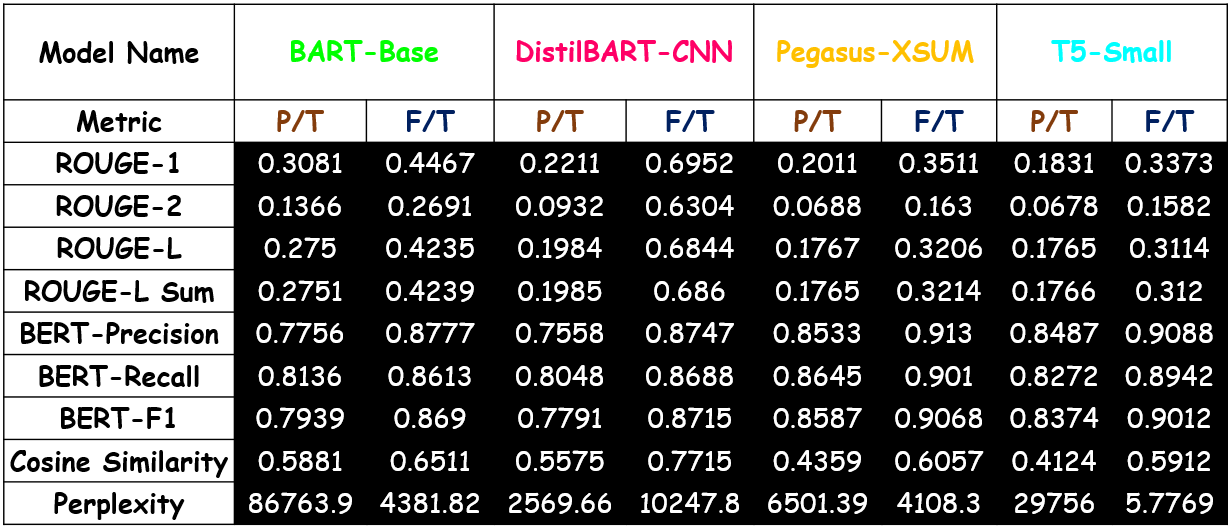
\includegraphics[width=\textwidth]{images/evaluation_table.png}
    \caption{Complete evaluation results: Pre-trained (P/T) vs Fine-tuned (F/T) across all four models and nine metrics}
    \label{fig:eval_table}
\end{figure}

\section{All-Model Cumulative Performance Comparison}

Figure~\ref{fig:all_comparison} shows the cumulative average of ROUGE-1, BERTScore F1, Cosine Similarity, and Perplexity across 1000 Q\&A pairs for all fine-tuned models.

\begin{figure}[H]
    \centering
    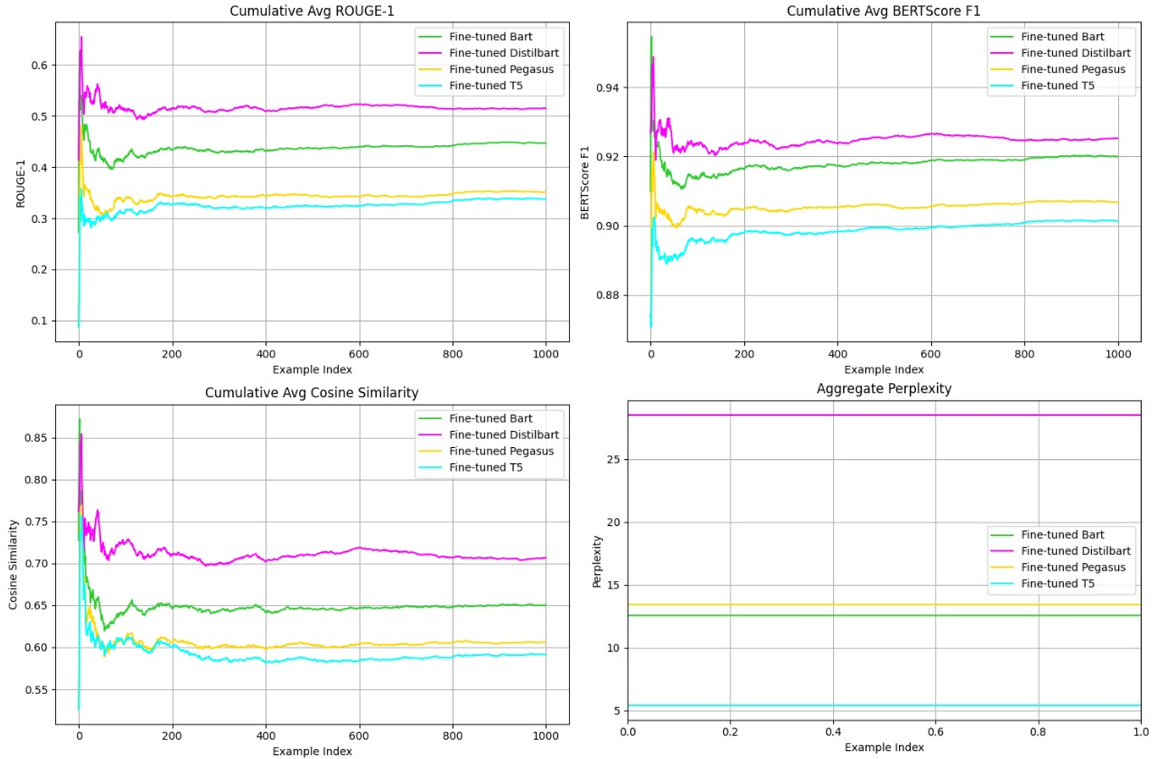
\includegraphics[width=\textwidth]{images/all_model_comparison.png}
    \caption{Cumulative average performance across 1000 Q\&A pairs — all four fine-tuned models compared across four metrics}
    \label{fig:all_comparison}
\end{figure}

Key observations from the cumulative plots:
\begin{itemize}
    \item DistilBART-CNN (pink/magenta) dominates ROUGE-1 and Cosine Similarity, stabilising around 0.51 and 0.70 respectively after the initial warm-up period.
    \item All models converge after approximately 100--150 examples, indicating stable generalisation.
    \item T5-Small (cyan) has near-flat perplexity at 5, dramatically outperforming the others in fluency.
    \item Pegasus-XSUM (yellow) maintains strong BERTScore F1, indicating consistent semantic output quality.
\end{itemize}

\section{Per-Model Analysis}

\subsection{BART-Base}

\begin{figure}[H]
    \centering
    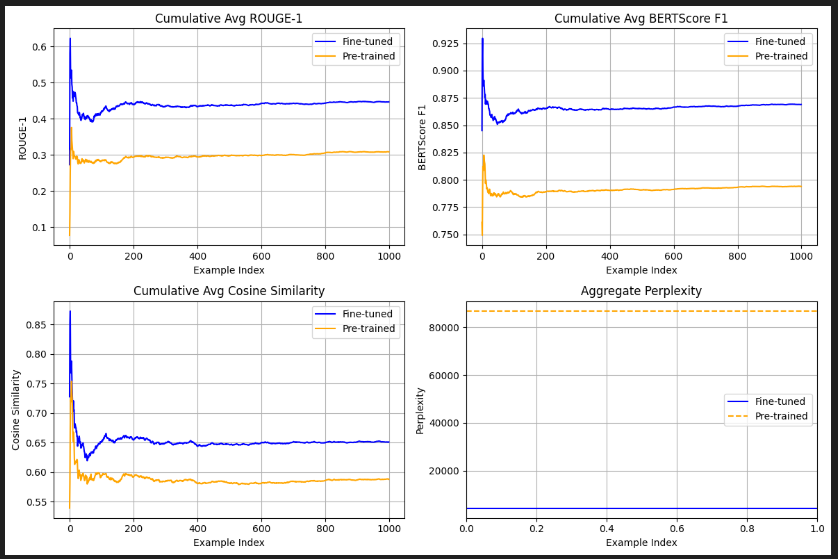
\includegraphics[width=\textwidth]{images/bartbase_output.png}
    \caption{BART-Base: Fine-tuned vs Pre-trained cumulative performance across all four metrics}
    \label{fig:bartbase}
\end{figure}

BART-Base shows consistent improvement after fine-tuning across all metrics. ROUGE-1 improves from 0.3081 to 0.4467 (+45\%). BERTScore F1 improves from 0.7939 to 0.8690. The perplexity drops dramatically from 86,763 to 4,381, though it remains the highest among fine-tuned models. BART-Base is the strongest general-purpose baseline in this study.

\subsection{DistilBART-CNN}

\begin{figure}[H]
    \centering
    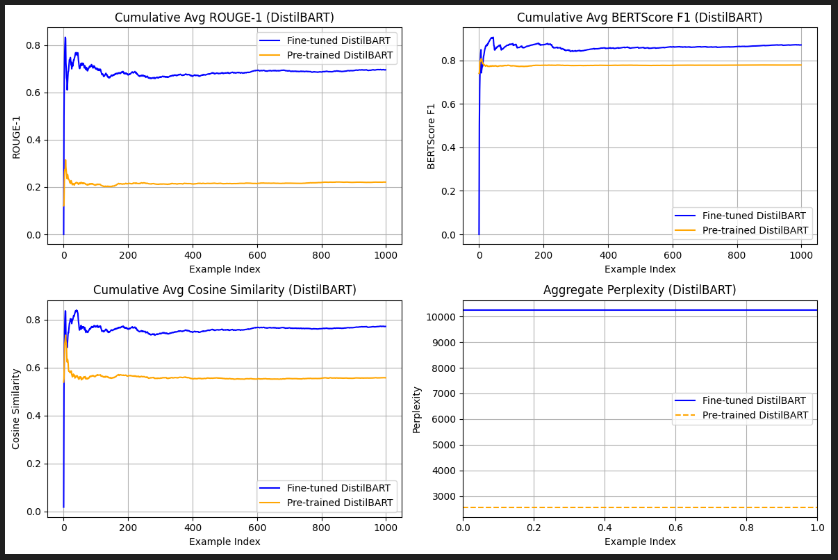
\includegraphics[width=\textwidth]{images/distilbart_output.png}
    \caption{DistilBART-CNN: Fine-tuned vs Pre-trained cumulative performance across all four metrics}
    \label{fig:distilbart}
\end{figure}

DistilBART-CNN shows the most dramatic improvement of any model. ROUGE-1 increases from 0.2211 to 0.6952 --- a $+214\%$ improvement. Cosine Similarity jumps from 0.5575 to 0.7715. This exceptional adaptability is likely because DistilBART-CNN was pre-trained on CNN/DailyMail news summarisation, a task structurally similar to scientific abstract summarisation, giving it a strong prior to build upon. It is the recommended model for summarisation tasks.

\subsection{Pegasus-XSUM}

\begin{figure}[H]
    \centering
    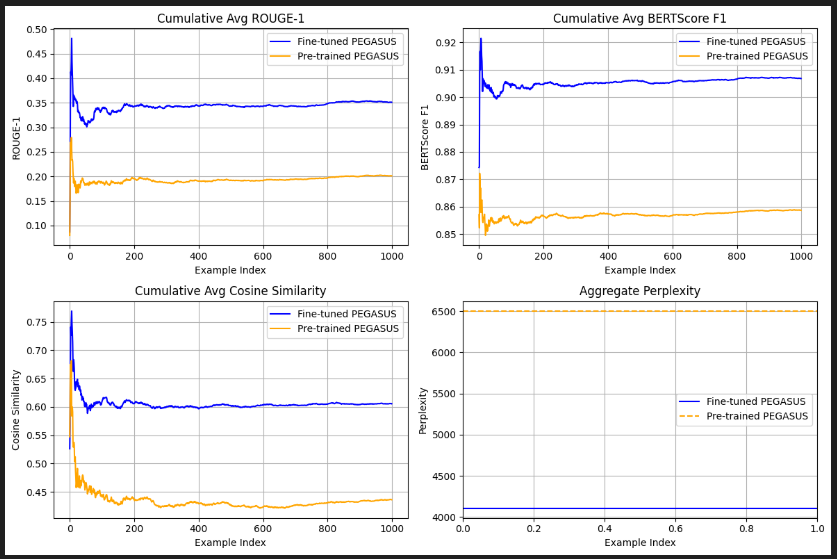
\includegraphics[width=\textwidth]{images/pegasus_output.png}
    \caption{Pegasus-XSUM: Fine-tuned vs Pre-trained cumulative performance across all four metrics}
    \label{fig:pegasus}
\end{figure}

Pegasus-XSUM achieves the highest BERTScore F1 of 0.9068 among all fine-tuned models, reflecting its strong semantic understanding. Its ROUGE scores are moderate because Pegasus tends to generate abstractive (paraphrased) outputs that are semantically correct but do not exactly match the reference wording --- this is precisely the trade-off between lexical and semantic metrics. Pegasus is the recommended model for tasks requiring semantic richness.

\subsection{T5-Small}

\begin{figure}[H]
    \centering
    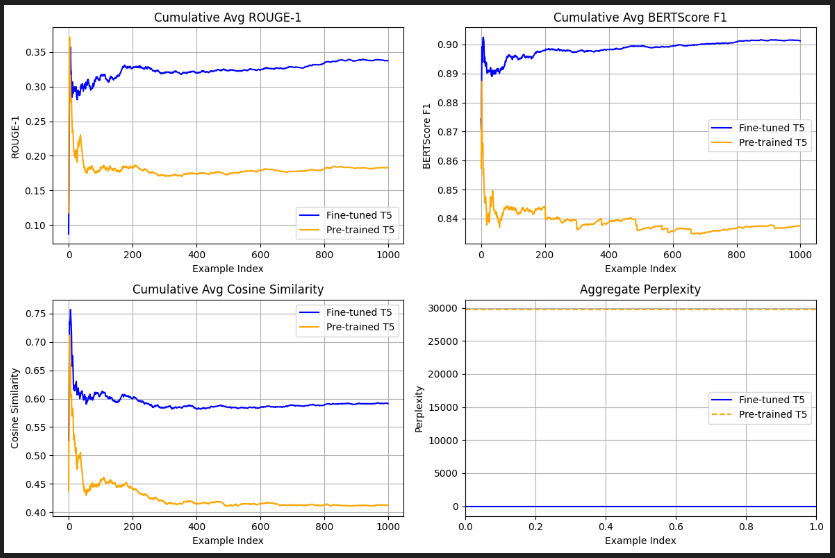
\includegraphics[width=\textwidth]{images/t5_output.png}
    \caption{T5-Small: Fine-tuned vs Pre-trained cumulative performance across all four metrics}
    \label{fig:t5}
\end{figure}

T5-Small achieves the lowest perplexity of all models --- 5.7769 --- a reduction from 29,756 pre-tuning. This represents the most dramatic fluency improvement in this study. Its BERTScore F1 of 0.9012 is the second highest. The relatively modest ROUGE scores (ROUGE-1: 0.3373) are explained by T5's tendency to paraphrase rather than copy: its answers are often semantically correct but worded differently from the reference. T5-Small is the recommended model for Q\&A tasks where fluency and naturalness are priorities.

\section{Cross-Model Comparison}

\begin{table}[H]
\centering
\caption{Model-Task Suitability Mapping}
\begin{tabular}{llll}
\toprule
\textbf{Model} & \textbf{Best Metric} & \textbf{Best Use Case} & \textbf{Key Strength} \\
\midrule
DistilBART-CNN & ROUGE-1: 0.6952 & Summarisation & Highest lexical overlap \\
Pegasus-XSUM & BERT-F1: 0.9068 & Semantic summarisation & Semantic richness \\
T5-Small & Perplexity: 5.77 & Q\&A tasks & Most fluent outputs \\
BART-Base & Balanced & General purpose & Consistent all-round \\
\bottomrule
\end{tabular}
\end{table}

All fine-tuned models outperformed their pre-trained baselines by substantial margins, confirming that domain-specific fine-tuning is essential for material informatics applications. Compared to a vanilla BERT baseline, fine-tuned models achieved BERT-F1 gains of $+12\%$ to $+38\%$.

% ════════════════════════════════════════════════════════════════════════════
\chapter{Conclusion}

This project successfully demonstrated that fine-tuned transformer-based NLP models can significantly accelerate knowledge extraction from graphene scientific literature. The key contributions of this work are:

\begin{enumerate}[leftmargin=*]
    \item \textbf{Domain-specific fine-tuning works}: All four models showed substantial performance improvements after fine-tuning on the Graphene Corpora, confirming that domain adaptation is essential for specialised scientific NLP tasks.

    \item \textbf{Task-model specialisation}: Different models excel at different tasks. DistilBART-CNN is best for summarisation (ROUGE-1: 0.6952), Pegasus-XSUM for semantic tasks (BERT-F1: 0.9068), and T5-Small for Q\&A and fluency (Perplexity: 5.77).

    \item \textbf{Efficient training under constraints}: The use of FP16, gradient accumulation, and gradient checkpointing enabled effective fine-tuning of large transformer models within Google Colab's GPU memory limitations.

    \item \textbf{Multi-metric evaluation}: Using four complementary metrics (ROUGE, BERTScore, Cosine Similarity, Perplexity) provided a comprehensive and nuanced understanding of model behaviour that no single metric could capture alone.
\end{enumerate}

The results lay critical groundwork for future research in deploying language models to accelerate materials discovery pipelines.

% ════════════════════════════════════════════════════════════════════════════
\chapter{Future Work}

Building on this project's foundations, the following directions are proposed for future work:

\begin{enumerate}[leftmargin=*]
    \item \textbf{Dataset expansion}: Incorporate Scopus corpora covering other 2D materials such as MoS\textsubscript{2}, h-BN, and perovskites to improve model generalisability beyond graphene.

    \item \textbf{Larger model variants}: Investigate BART-Large and T5-Base, which have greater capacity and may yield further performance gains given sufficient computational resources.

    \item \textbf{Retrieval-Augmented Generation (RAG)}: Integrate a retrieval mechanism to allow the model to dynamically pull in relevant papers during inference, enabling real-time responses to emerging research questions.

    \item \textbf{Web deployment}: Develop a web-based interface allowing researchers to directly query the graphene knowledge base through a conversational Q\&A bot.

    \item \textbf{Knowledge graph integration}: Link extracted entities and relationships from abstracts into a materials science knowledge graph to support structure--property prediction tasks.
\end{enumerate}

% ════════════════════════════════════════════════════════════════════════════
\chapter*{References}
\addcontentsline{toc}{chapter}{References}

\begin{enumerate}[leftmargin=*]
    \item Lewis, M., Liu, Y., Goyal, N., Ghazvininejad, M., Mohamed, A., Levy, O., Stoyanov, V., \& Zettlemoyer, L. (2020). BART: Denoising Sequence-to-Sequence Pre-training for Natural Language Generation, Translation, and Comprehension. \textit{Proceedings of the 58th Annual Meeting of the Association for Computational Linguistics (ACL 2020)}. \url{https://arxiv.org/abs/1910.13461}

    \item Zhang, J., Zhao, Y., Saleh, M., \& Liu, P. (2020). PEGASUS: Pre-training with Extracted Gap-sentences for Abstractive Summarization. \textit{International Conference on Machine Learning (ICML 2020)}. \url{https://arxiv.org/abs/1912.08777}

    \item Raffel, C., Shazeer, N., Roberts, A., Lee, K., Narang, S., Matena, M., Zhou, Y., Li, W., \& Liu, P. J. (2020). Exploring the Limits of Transfer Learning with a Unified Text-to-Text Transformer. \textit{Journal of Machine Learning Research, 21}(140), 1--67. \url{https://arxiv.org/abs/1910.10683}

    \item Sanh, V., Debut, L., Chaumond, J., \& Wolf, T. (2019). DistilBERT, a Distilled Version of BERT: Smaller, Faster, Cheaper and Lighter. \textit{NeurIPS 2019 Workshop on Energy Efficient Deep Learning}. \url{https://arxiv.org/abs/1910.01108}

    \item Zhang, T., Kishore, V., Wu, F., Weinberger, K. Q., \& Artzi, Y. (2020). BERTScore: Evaluating Text Generation with BERT. \textit{International Conference on Learning Representations (ICLR 2020)}. \url{https://arxiv.org/abs/1904.09675}

    \item Reimers, N., \& Gurevych, I. (2019). Sentence-BERT: Sentence Embeddings using Siamese BERT-Networks. \textit{Proceedings of the 2019 Conference on Empirical Methods in Natural Language Processing (EMNLP 2019)}. \url{https://arxiv.org/abs/1908.10084}

    \item Wolf, T., Debut, L., Sanh, V., Chaumond, J., Delangue, C., Moi, A., \& others. (2020). Transformers: State-of-the-Art Natural Language Processing. \textit{Proceedings of the 2020 Conference on Empirical Methods in Natural Language Processing: System Demonstrations}. \url{https://arxiv.org/abs/1910.03771}
\end{enumerate}

\end{document}
